\documentclass[10pt,conference,letterpaper]{IEEEtran}
%\documentclass[10pt,journal,cspaper, compsoc]{IEEEtran}


\usepackage{times,amsmath,epsfig}
\usepackage{balance}  % for  \balance command ON LAST PAGE  (only there!)
\usepackage{graphicx}
\usepackage{comment}
\usepackage{amssymb}
\usepackage{subfigure}
\usepackage{url}
\usepackage{times,epsfig,amsfonts,graphicx}
\usepackage{cite}
\usepackage{color}
\usepackage{savesym}
\usepackage{algorithm}
\usepackage{algorithmic}
\usepackage{verbatim}
\usepackage{multirow}
\usepackage{epsf}

%\usepackage[sorting=none]{biblatex}

\renewcommand{\algorithmicrequire}{\textbf{Input:}}
\renewcommand{\algorithmicensure}{\textbf{Output:}}

\definecolor{zhecolor}{rgb}{0,0.5,0.8}
\newcommand{\zhe}[1]{\textcolor{zhecolor}{#1}}
\definecolor{mycolor}{rgb}{0.7,0,0}
\newcommand{\choi}[1]{\textcolor{mycolor}{#1}}
\newcommand{\sxyin}[1]{\textcolor{red}{#1}}
\newcommand{\red}[1]{\textcolor{red}{#1}}
\newcommand{\eat}[1]{}
\newcommand{\stab}{\rule{0pt}{8pt}\\[-2.0ex]}
\newcommand{\ltab}{\stab \stab }
%\newtheorem{definition}{Definition}[section]
%\newtheorem{example}{Example}[section]
%\newtheorem{theorem}{Theorem}[section]
%\newtheorem{proposition}{Proposition}[section]
\newcommand{\tab}{\text{    } \text{    } \text{    }}


\newcommand{\SYN}{ {\tt SYN}}
\newcommand{\maxintr}{ I_{{\tt max}} }
\newcommand{\pphop}{${\tt pp}$-${\tt 2}$-${\tt hop}$}
\newcommand{\hop}{${\tt 2}$-${\tt hop}$}
\newcommand{\unifylin}{{\tt unifyLin}}
\newcommand{\unifyIS}{{\tt unifyIS}}
\newcommand{\next}{{\tt getNext}}
\newcommand{\linmax}{\lin_{\tt max}}
\newcommand{\loutmax}{\lout_{\tt max}}
\newcommand{\madd}{${\tt MASN}$}
\newcommand{\nadd}{${\tt Naive}$}
\newcommand{\uls}{${\tt ULS}$}
\newcommand{\mvc}{${\tt MVC}$}
\newcommand{\f}{f}
\newcommand{\we}{w_e}
\newcommand{\fe}{f_e}
\newcommand{\re}{R_e}
\newcommand{\hash}{h}
\newcommand{\encrypt}{{\tt E}}
\newcommand{\lin}{{\tt Lin}}
\newcommand{\lout}{{\tt Lout}}
\renewcommand{\line}{{\tt Lin^e}}
\newcommand{\loute}{{\tt Lout^e}}
\newcommand{\lins}{{\tt Lin^s}}
\newcommand{\louts}{{\tt Lout^s}}
\renewcommand{\to}{\rightsquigarrow}
\newcommand{\g}{G}
\newcommand{\q}{q}
\newcommand{\DAG}{${\tt DAG}$}
\newcommand{\fnc}{{\cal F}}


\renewcommand{\l}{L}
\renewcommand{\r}{R}
\newcommand{\e}{E}
\newcommand{\SP}{${\cal SP}$}

\newcommand{\ratio}{r}
\newcommand{\maxDC}{ {\tt maxDensCover} }
\newcommand{\maxC}{ {\tt maxSetCover} }
\newcommand{\maxIS}{ {\tt maxISCover} }

\newcommand{\tightfloat}{\setlength{\textfloatsep}{2pt}}


\begin{document}

% Strong
\title{Supporting Compression in Privacy Preserving Reachability Query}

\author{Peipei YI, Zhe FAN, Shuxiang YIN\\
{\tt csppyi,zhe@comp.hkbu.edu.hk ??}

\IEEEcompsocitemizethanks{\IEEEcompsocthanksitem Peipei Yi and Byron Choi are with the Department of Computer Science, Hong Kong Baptist University, China. \protect\\
E-mail: csppyi, bchoi@comp.hkbu.edu.hk
}
\\
Hong Kong Baptist University
\thanks{}}
\IEEEcompsoctitleabstractindextext{}
%
\maketitle


\begin{abstract}
Due to the massive volume of graph data from a wide range of recent
applications and resources required to process numerous queries at
large scale, it is becoming economically appealing to outsource graph
data to a third-party service provider (\SP), to provide query
services. However, \SP\ cannot always be trusted.  Hence, data owners
and query clients may prefer not to expose their data graphs and
queries. This paper studies privacy preserving query services for a
fundamental query for graphs namely the reachability query where {\em
  both} clients' queries and the structural information of the owner's
data are protected. We propose {\em privacy preserving 2-hop labeling}
(\pphop) where the queries are computed in an encrypted domain and the
input and output sizes of any queries are indistinguishable. We
analyze the security of \pphop\ with respect to ciphertext only and
size based attacks. We verify the performance of \pphop\ with an
experimental study on both synthetic and real-world datasets.
\end{abstract}
%\vspace{-1ex}
\section{Introduction}
\label{sec:intro}


% reachability query application
There is a wide range of emerging applications of
graph-structured data, {\it e.g.}, bioinformatics, communication
networks, social networks, web topology and semi-structured data. Many graph queries have been proposed to retrieve such graph
data.
%%
% problem of management of data and query
%%
% Byron: in reality, graphs are not managed by users.
However, as the volume of graph data is increasing at an unprecedented rate,
hosting efficient query services has become a technically challenging task.  The
{\em owners} of graph data may not always be equipped with the expertise
required to provide such services and therefore may
%%
% query services
%%
employ {\em query service providers} (\SP s) to host {\em query services}, which
are often supported by high performance computing. Security (such as
the confidentiality of messages exchanged) has been stated as one of the
attributes of Quality of Services (QoS) \cite{issues}, as \SP\ s cannot always be
trusted. This attribute may influence the willingness of both data owners and query clients to use \SP's services.


% motivate the query together with privacy
Take the reachability query ---  one of the most fundamental and popular graph queries
\cite{cohen, ferrari, sigmod2012, grail, gripp, 3hop, pathhop, hopi, chengjf1,
chengjf2, byron, cikmlabel, bitcompression, pathtree} --- as an example:  {\em
Given two nodes $u$ and $v$ of a graph, the reachability query is used to test if $v$
is reachable from $u$ or not}.
% privacy problem of employment of query services 
A query client may prefer not to expose his/her reachability query to an \SP.
On the other hand, the data owner may prefer that the \SP\ not be able to infer
the structure of their graph data. Therefore, the query results must be
protected as malicious \SP s can exploit the results from multiple queries to
infer the graphs' structures.



\stab
\noindent {\bf Motivating example.} Consider a pharmaceutical company
whose revenue depends mostly on the invention of Health Care Products,
illustrated in Fig.~\ref{fig:overview}. The company may have
discovered new compounds for a new product. To save laboratory
experiments, it may query the compounds from web-accessible biological
pathway networks (such as \cite{biology}) to understand the compounds'
characteristics, such as whether it is possible for the compounds to
form other compounds via any chemical reactions (reachability in the
network). However, on the one hand, the company does not want the
\SP\ to know about the queries (the compounds), as it may apply for
patents for the synthesis. On the other hand, the owner of the pathway
networks may not only lack the experience to host query services but
also be reluctant to release the networks to the public.
Alternatively, the owner is willing to release a license only to paid
users.  Therefore, it is crucial to protect {\em both} the queries and
the network from the \SP.



\begin{figure}[t]
\begin{minipage}[t]{0.5\linewidth}
\centering
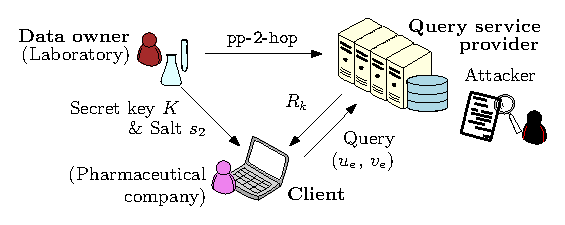
\includegraphics[width=2.2in]{./example/system.eps}
\vspace{-2ex}
\caption{Overview of the system model}
\label{fig:overview}
\end{minipage}%
\begin{minipage}[t]{0.5\linewidth}
\centering
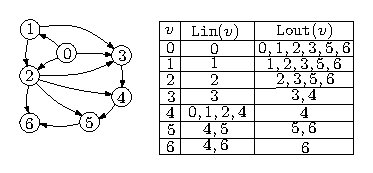
\includegraphics[width=1.6in]{./example/graph.eps}
\vspace{-4ex}
\caption{A (partial) schematic of a biological network  (LHS) and its \hop\ labeling (RHS)}
\label{fig:2hop}
\end{minipage}
%\vspace{-6ex}
\end{figure}

\stab
% Problem statement
This paper studies the problem of {\em evaluating the reachability
  query at an \SP\ without compromising the privacy of the
  reachability of the query nodes and the graph structure under
  cipertext-only and size-based attacks, in the paradigm of query
  services} (to be detailed with Fig.~\ref{fig:overview} in
Sec.~\ref{sec:preliminary}). To our knowledge, this has not been  addressed before.



% related reachability works in the literature (in light of privacy preservation)
There have been many recent studies  on efficient reachability query ({\it
e.g.}, \cite{pathtree, bitcompression,grail, gripp, ferrari,3hop, pathhop,
sigmod2013, hopi, chengjf1 ,chengjf2, byron}). Jin et al. \cite{sigmod2012}
show that these studies can be roughly categorized into {\em transitive closure
compressions}, {\em refined online search} and {\em hop labeling}. The first
two categories suffer from high storage costs and require
online searches, respectively (to be discussed in
Sec~\ref{subsec:related:reach}).
% adopt and motivate 2hop
In this paper, we propose our techniques based on hop  labeling
\cite{cohen}, in particular \hop\ labeling. The benefits of adopting \hop\ labeling are
threefold. Firstly, the structures of \hop\ labels are simple, where
each node is associated with two sets of nodes called $\lin$ and
$\lout$. Secondly, the query evaluation with \hop\ labeling is
an intersection between an $\lin$ and an $\lout$. Such simple
structure and algorithm make privacy
preservation plausible. Thirdly, \hop\ labeling is an active research
topic. The recent works on large graph  partitioning ({\it e.g.}, \cite{chengjf2}),
compression ({\it e.g.}, \cite{chengjf1}) and maintenance ({\it e.g.},
\cite{hopi,byron}) of \hop\ labeling can be readily adopted.




% the challenges and our solutions
% Byron: your methodologies
% addition of surrogate nodes
This paper proposes \pphop\ ({\em privacy preserving \hop}), which adopts
\hop\ labeling. 
%%%%
Firstly, 
the evaluation of each query on \hop\ labeling only involves an intersection between
two sets of center nodes.  Hence, we minimize the size of the
maximum cardinality of the intersection results and add {\em minimal}
artificial nodes (called surrogate nodes) to $\lin$s and $\lout$s such
that the intersection results for all possible queries are of the {\em
  same} size. We  unify each of the $\lin$ and $\lout$
labels such that the difference of the label set sizes are
within a user-defined parameter.
%%%%
Secondly, we encrypt the \hop\ labels, after adding surrogate nodes
and evaluate queries in the encrypted domain. We analyze the privacy
of \pphop.
% encryption of the index optimization
\eat{For optimization, we propose a heuristic function to minimize the maximum
cardinality of the intersection during query evaluation. }



% contribution
\noindent The contributions of this paper are summarized as follows.
\vspace{-1ex}
\begin{itemize}%\addtolength{\itemsep}{-0.3\baselineskip}

        \item We propose algorithms to  unify the sizes of \hop\ labels and the
            query result sizes; \eat{realize minimum addition
            of the surrogate nodes in 2-hop labeling;}

        \item We propose private query
            processing over the  encrypted \hop\ labels;

        \item We propose  a new heuristic \hop\ construction that yields \hop\
            labeling that minimizes the intermediate results in private query
            processing; and

        \item We conduct an empirical study to confirm that our techniques are efficient.
\end{itemize}
\vspace{-1ex}

The rest of this paper is organized as follows. We
introduce some related work in Sec.~\ref{sec:related}. We then present the
background, the problem and the overview of our solution in Sec.~\ref{sec:preliminary}. We
propose \pphop, the index construction, optimization  and query processing in
Sec.~\ref{sec:preprocessing}. We conduct a  privacy analysis in
Sec.~\ref{sec:analysis}. We present an experimental evaluation in
Sec.~\ref{sec:exp}. We end this paper with the conclusion in
Sec.~\ref{sec:conclusion}.






















\section{Problem Formulation}
\label{sec:formulation}

This section formulates the problem studied and gives an overview of our solution.


\subsection{Data Model}
We consider {\em directed
  node-labeled graphs}.  A graph is denoted as $\g$, and $V(\g)$ and
$E(\g)$ are the node and edge sets of $\g$, respectively.  Since the
reachability information of nodes in a strongly connected component is identical, we assume directed acyclic graphs
(\DAG), for presentation brevity. A reachability query takes two nodes
$u$ and $v$ as input, denoted as $u \leadsto v$, and returns true {\it
  iff} $v$ is reachable from $u$.


\subsection{System Model}
\label{subsec:system_model}
We follow the system model that is
commonly used in the literature of database outsourcing, presented in
Fig.~\ref{fig:overview}.  The model consists of three parties:
%

\begin{itemize}%\addtolength{\itemsep}{-0.5\baselineskip}
% 1
\item {\em Data owner}: An owner owns the graph data and computes the
    privacy preserving \hop\ labeling offline {\em once}. It  outsources them to the
    service provider and delivers query clients a salt $s_2$ to encrypt queries
    and the secret key $K$ to decrypt results;  
% 2
\item {\em Service provider} (\SP): The \SP\ has high computational
  utility such as cloud computing. The \SP\ handles massive query
  requests over the encrypted data on behalf of the data owner and
  returns the encrypted results to clients; and
% 3
\item {\em Client}: A client encrypts a query using $s_2$, sends the
  encrypted query to the \SP\ and decrypts the result with
  $K$. We assume that the clients and \SP\ do not collude.
%
\end{itemize}


\subsection{Privacy Target}
Our privacy target is
required to keep the following two pieces of information private from {\em attackers}
using the two attacks defined in the attack model: 
%
\begin{itemize}%\addtolength{\itemsep}{-0.5\baselineskip}
    %
    \item {\em Reachability of the query nodes} a.k.a the query result. In
        particular, given a reachability query $u \leadsto v$, attackers cannot
        infer whether $u$ can reach to $v$; and
    %
    \item {\em Graph structure} a.k.a. the topology of the data graph, {\it
        e.g.}, the existence of an edge.
    %
\end{itemize} 


\subsection{Attack Model}
We assume the \SP s are {\em
  honest-but-curious}. The attackers  may be the
\SP\ or another adversary hacking the \SP.  For simplicity, we often {\em term the
  attackers as the \SP}. We assume that the \SP\ can adopt the
following attacks.\footnote{There are many other
  attacks in the literature.  We do not consider them all in
  one approach.}  
%
\begin{itemize}
    %
    \item {\em Ciphertext only attack}, where the \SP\ can
        access only the ciphertext (encrypted graph data) and does not know what
        their original graph is; and 
    %
    \item {\em Size based attack}, where the \SP\ attempts to infer the two pieces of private
        information from the sizes of the data and the query
        results.
    %
\end{itemize} 


To sum up, ...
	% problem formulation
\section{Preliminary}
\label{sec:preliminary}

\subsection{\hop}
\label{subsec:hop}

\subsubsection{Background of Cryptography}
\label{subsec:encryption}

As motivated in Sec~\ref{sec:intro}, we shall process queries on
encrypted \hop\ labels. In this paper, we exploit the following two techniques.

\stab
\noindent {\bf One-way collision-resistant hash function.} A one-way
collision-resistant hash function, denoted as $\hash()$, is to determine a hash
value $\hash(m)$ from a given data value $m$. It involves two properties. (1)~{\em One-way}, which indicates that it is infeasible to determine the preimage
$m$ of a given $\hash(m)$; and (2) {\em Collision-resistant}, which refers that
it is infeasible to find two different data values with the same hash value. One
of the state-of-the-art functions is SHA-1 \cite{sha}.

In the literature, a {\em salt} $s$ is commonly supported by one-way
collision-resistant functions, which is an additional input to a function,
denoted as $\hash_s()$. Given different salts, the hash values produced by
$\hash_s()$ are different. In other words, $\hash_{s_1}(m) \neq \hash_{s_2}(m)$
if $s_1 \neq s_2$, and $\hash_{s_1}(m) = \hash_{s_2}(m)$ if $s_1 = s_2$. In this
paper, we use two different salts as a part of the secret keys of the data
owner.

\stab
\noindent {\bf Multiplicative homomorphic encryption function.} A
multiplicative homomorphic encryption function is denoted as
$\encrypt(\cdot)$.  The multiplications in its encrypted domain are
homomorphic to those in the plaintext. In particular, given the
ciphertext $\encrypt(m_1)$ and $\encrypt(m_2)$, one can compute
$\encrypt(m_1 \times m_2)$ from the ciphertext and obtain the result of
$m_1 \times m_2$ by a decryption using a secret key $K$. One of the
representative methods in the literature is Elgamal \cite{elgamal}. It
is worth-noting that Elgamal ensures high randomness in the
ciphertext. In other words, the encrypted values of the same data
values are different from each other, {\it i.e.}, $\encrypt(m_1) \neq
\encrypt(m_2)$ even if $m_1 = m_2$. This is crucial to applications
where the domain of the plaintext is small.

\section{Overview}
\section{Biclique Cover}
\label{sec:biclique}

Definition - Unify Intersection Size

Greedy Algorithm

\begin{algorithm}[t]
\caption{Greedy Find Maximum Clique}
\label{alg:greedy_clique}
\algsetup{linenosize=\small}
\begin{algorithmic}[1]
%\begin{small}
\REQUIRE an undirected graph $G$
\ENSURE maximum clique $C$

\STATE C \GETS \varnothing

\REQUIRE 2-hop labeling $\lout$ and $\lin$
\ENSURE $\louts$ and $\lins$

\STATE Initialize a virtual surrogate node set $D_w = [ d_1, d_2, \cdots ]$
\stab
\stab
\STATE create a priority queue $Q_u$ (sorted by $|\lin|$($u$) in desc. order) for $V(\g)$
\STATE {\bf while} $u \not = {\tt null}$, where $u$ $\leftarrow Q_u$.$\next$() 
\stab
\stab
\STATE \tab {\bf for each} $d_i \in D_w$  //reuse surrogates
\stab
\stab
\STATE \tab  \tab create a priority queue $Q_v$  (sorted by $| \lout(u) \cap \lin(v) |$ \\
\tab \tab in asc. order) for $V(\g)$
\STATE \tab \tab {\bf while} $v$$\not =$${\tt null}$, where $v \leftarrow Q_v$.$\next$() $\wedge$ \\
\tab \tab \tab $|\lout(u) \cap \lin(v) | < \maxintr$ \\
\stab 
\stab 
\tab \tab \tab  //{\small if the {\em intersection constraint} is satisfied.}
\STATE \tab \tab \tab  {\bf if} $\psi$(\hop, $u$, $v$, $d_i$) is true  
\STATE \tab \tab \tab \ \ $\lout(u)$$\leftarrow$$\lout(u)$$\cup$$\{d_i\}$; $\lin(v)$$\leftarrow$$\lin(v)$$\cup$$\{d_i\}$ 
\stab
\STATE {\bf return} ($\lout$, $\lin$) {\bf as} ($\louts$, $\lins$)

%\end{small}
\end{algorithmic}
\end{algorithm}

Lecture Bound

\section{Analysis of Privacy}
\label{sec:analysis}

In this section, we provide an analysis of the privacy under the
assumptions of our attack model, {\it i.e.}, the size based attack and
ciphertext only attack (stated in Sec.~\ref{sec:preliminary}).

\section{Experimental Evaluation}
\label{sec:exp}

In this section, we present the experimental evaluation that verifies
the performance of our proposed techniques and the effectiveness of our
optimization.

\subsection{Experimental Setup}
\label{subsec:expsetup}


\noindent {\bf Running platform.} We conducted all experiments using a machine
with Intel Core i3-2310 2.10GHz CPU and 4G RAM running Windows 7 OS.  All
algorithms were implemented using ++ basCed on the implementation of \hop\
labelings provided by R.Bramandia et al. \cite{byron}. The hash function ($\hash_{s_1}$
and $\hash_{s_2}$) was  160-bit SHA-1 using two different salts. %and MD5 The
The encryption  $\encrypt$ was 1024-bit Elgamal \cite{elgamal}.

\stab
\noindent {\bf Datasets.} We used three synthetic datasets (denoted as \SYN) and four
real-world datasets. Some of their characteristics are shown in
Table~\ref{table:syndata}. The synthetic datasets were all scale-free graphs,
which are popular in experimentation. The generator used was provided by Choi
et al. \cite{generator}. We controlled the sizes and densities of the graphs by
setting $\alpha = 0.27$ and $\beta = 10$.  The real-world datasets are all
publicly available.\footnote{\scriptsize
YEAST: http://vlado.fmf.uni-lj.si/pub/networks/data/bio/Yeast/Yeast.htm \\
ODLTS: http://vlado.fmf.uni-lj.si/pub/networks/data/dic/odlis/Odlis.htm \\
ERDOS: http://vlado.fmf.uni-lj.si/pub/networks/data/Erdos/Erdos02.net \\
ROGET: http://vlado.fmf.uni-lj.si/pub/networks/data/dic/roget/Roget.htm
} % footnote of real data



\vspace{-2ex}
\section{Related Work}
\label{sec:related}
\vspace{-2ex}

In this section, we present some related works on security of
graph queries. 

%% We then introduce the current state of privacy preserving
%% graph query. We end this section with the introduction of the approaches for
%% reachability query.

\stab
\noindent{\bf Authentication of graph queries.} Query authentication
is a security problem where the \SP\ cannot be trusted. It requires the client to verify the correctness
of the data graphs returned.  Kundu et
al. \cite{auth_graph_wo_leaking,signature, forest} focus on the verification of the {\em authenticity} of a
{\em given portion of data} (subtree/subgraph that users' have the
right to access to) without leakage of extraneous information of the
data (tree/graph/forest). They optimize the signature needed
\cite{forest, signature}. 
Zhe et al. \cite{zhe} propose an efficient authenticated subgraph query
services framework under the outsourced graph databases system. 
In comparison, the input of our problem is a
reachability query not a subgraph for verification. Our problem
focuses on {\em protecting both the query and its answer from \SP s}.

\stab
\noindent{\bf Privacy preserving graph query.} He et
al. \cite{edgeprivacy} analyze the node reachability of the graph
data, with the preservation of edge privacy. Unfortunately, the method
reveals the reachability of the query nodes and partial structure of
the graph data to the \SP.  Gao et al.  \cite{Jeffery} propose
neighborhood-privacy protected shortest distance in the paradigm of
cloud computing. This aims to preserve all the neighborhood connections
and the shortest distances between each pair of nodes in outsourced
graph data. When this work is directly applied to reachability
queries, some information about the graph structure and the
reachability of the query nodes are still exposed to the \SP.

Mouratidis et al.  \cite{PIR+SP} determine the shortest path of the query
nodes with no information leakage by using the PIR \cite{PIR}
protocol.  Firstly, the high computational cost of PIR is still a
concern. Secondly, the PIR approach requires the transfer of the
same amount of data for every query, which can be large. Reachability
queries are simple (yet fundamental) queries and do not require the use of
the costly PIR method.  Cao et al. \cite{ICDCS} propose to
support subgraph query over an encrypted database of small graphs.
Their work protects the query privacy, index privacy and feature
privacy. However, reachability queries cannot be expressed as subgraph
queries. Karwa et al. \cite{subgraph+count} present an efficient
algorithm for outsourcing useful statistics of graph data by
protecting the edge {\em differential privacy} and they
support counting queries but not reachability queries.

\stab
\noindent{\bf Approaches for reachability
  query.}\label{subsec:related:reach} Numerous approaches for
reachability query have been proposed recently in the literature. Jin
et al. \cite{sigmod2012} recently discuss the approaches based on
three main categories: {\em transitive closure compressions}, {\em
  refined online search} and {\em hop labeling}. The seminal
\hop\ labeling is proposed by Cohen et al. \cite{cohen} and further optimized by many studies \cite{hopi,chengjf1, chengjf2}.  Due to the simple
structure of the \hop\ labeling approach and the simple query
evaluation, in this paper, we propose our techniques based on the
\hop\ labeling approach.


% 1

%% (i) Transitive closure compressions ({\it e.g.},\cite{sigmod1989,
%%   pathtree, bitcompression}) exhibit the best query
%% performances. It is known that their storage costs are the
%% highest and often impractical. 

%% (ii) Refined online search ({\it
%%   e.g.}, \cite{grail, gripp, ferrari}) utilizes some online
%% search strategies to answer reachability query. However, online
%% searches ({\it e.g.}, DFS and BFS) carry the information of
%% graph structures and it is not clear how  they can be adopted. 

%% (iii) The seminal \hop\ labeling is proposed by Cohen \cite{cohen}.
%% Various interesting works of \hop\ are recently proposed to enhance
%% query performances ({\it e.g.}, \cite{3hop, pathhop, sigmod2013})
%% and maintenance performances \cite{byron}. A stream of previous work
%% on \hop\ focuses on optimizing the sizes of \hop\ and its high
%% construction cost \cite{hopi,chengjf1, chengjf2}. Cheng et
%% al. \cite{sigmod2013} proposes a topological folding labeling scheme
%% that establishes an \hop\ like labeling.

%% Each vertex is assigned two sets of vertices (\hop\ labels)
%% only. Due to the simple structure of the \hop\ labeling approach and
%% the simple query evaluation, in this paper, we propose our techniques
%% based on the \hop\ labeling approach.




%% There are many studies on privacy preserving graph publication
%% undertaking the structure anonymization approach ({\it e.g.},
%% \cite{1-neighborhood, k-degree, k-automorphism,
%%   k-isomorphism}). Structural information of graphs are changed by
%% anonymization and it is not clear how to support reachability
%% queries. Due to space limitation, we do not include detailed
%% comparisons with these studies.


\section{Conclusion and Future Work}

\end{document}
